% GNUPLOT: LaTeX picture with Postscript
\begingroup
  \makeatletter
  \providecommand\color[2][]{%
    \GenericError{(gnuplot) \space\space\space\@spaces}{%
      Package color not loaded in conjunction with
      terminal option `colourtext'%
    }{See the gnuplot documentation for explanation.%
    }{Either use 'blacktext' in gnuplot or load the package
      color.sty in LaTeX.}%
    \renewcommand\color[2][]{}%
  }%
  \providecommand\includegraphics[2][]{%
    \GenericError{(gnuplot) \space\space\space\@spaces}{%
      Package graphicx or graphics not loaded%
    }{See the gnuplot documentation for explanation.%
    }{The gnuplot epslatex terminal needs graphicx.sty or graphics.sty.}%
    \renewcommand\includegraphics[2][]{}%
  }%
  \providecommand\rotatebox[2]{#2}%
  \@ifundefined{ifGPcolor}{%
    \newif\ifGPcolor
    \GPcolorfalse
  }{}%
  \@ifundefined{ifGPblacktext}{%
    \newif\ifGPblacktext
    \GPblacktexttrue
  }{}%
  % define a \g@addto@macro without @ in the name:
  \let\gplgaddtomacro\g@addto@macro
  % define empty templates for all commands taking text:
  \gdef\gplbacktext{}%
  \gdef\gplfronttext{}%
  \makeatother
  \ifGPblacktext
    % no textcolor at all
    \def\colorrgb#1{}%
    \def\colorgray#1{}%
  \else
    % gray or color?
    \ifGPcolor
      \def\colorrgb#1{\color[rgb]{#1}}%
      \def\colorgray#1{\color[gray]{#1}}%
      \expandafter\def\csname LTw\endcsname{\color{white}}%
      \expandafter\def\csname LTb\endcsname{\color{black}}%
      \expandafter\def\csname LTa\endcsname{\color{black}}%
      \expandafter\def\csname LT0\endcsname{\color[rgb]{1,0,0}}%
      \expandafter\def\csname LT1\endcsname{\color[rgb]{0,1,0}}%
      \expandafter\def\csname LT2\endcsname{\color[rgb]{0,0,1}}%
      \expandafter\def\csname LT3\endcsname{\color[rgb]{1,0,1}}%
      \expandafter\def\csname LT4\endcsname{\color[rgb]{0,1,1}}%
      \expandafter\def\csname LT5\endcsname{\color[rgb]{1,1,0}}%
      \expandafter\def\csname LT6\endcsname{\color[rgb]{0,0,0}}%
      \expandafter\def\csname LT7\endcsname{\color[rgb]{1,0.3,0}}%
      \expandafter\def\csname LT8\endcsname{\color[rgb]{0.5,0.5,0.5}}%
    \else
      % gray
      \def\colorrgb#1{\color{black}}%
      \def\colorgray#1{\color[gray]{#1}}%
      \expandafter\def\csname LTw\endcsname{\color{white}}%
      \expandafter\def\csname LTb\endcsname{\color{black}}%
      \expandafter\def\csname LTa\endcsname{\color{black}}%
      \expandafter\def\csname LT0\endcsname{\color{black}}%
      \expandafter\def\csname LT1\endcsname{\color{black}}%
      \expandafter\def\csname LT2\endcsname{\color{black}}%
      \expandafter\def\csname LT3\endcsname{\color{black}}%
      \expandafter\def\csname LT4\endcsname{\color{black}}%
      \expandafter\def\csname LT5\endcsname{\color{black}}%
      \expandafter\def\csname LT6\endcsname{\color{black}}%
      \expandafter\def\csname LT7\endcsname{\color{black}}%
      \expandafter\def\csname LT8\endcsname{\color{black}}%
    \fi
  \fi
  \setlength{\unitlength}{0.0500bp}%
  \begin{picture}(15306.00,10204.00)%
    \gplgaddtomacro\gplbacktext{%
      \csname LTb\endcsname%
      \put(814,704){\makebox(0,0)[r]{\strut{} 4}}%
      \put(814,1686){\makebox(0,0)[r]{\strut{} 6}}%
      \put(814,2668){\makebox(0,0)[r]{\strut{} 8}}%
      \put(814,3650){\makebox(0,0)[r]{\strut{} 10}}%
      \put(814,4632){\makebox(0,0)[r]{\strut{} 12}}%
      \put(814,5615){\makebox(0,0)[r]{\strut{} 14}}%
      \put(814,6597){\makebox(0,0)[r]{\strut{} 16}}%
      \put(814,7579){\makebox(0,0)[r]{\strut{} 18}}%
      \put(814,8561){\makebox(0,0)[r]{\strut{} 20}}%
      \put(814,9543){\makebox(0,0)[r]{\strut{} 22}}%
      \put(946,484){\makebox(0,0){\strut{} 0}}%
      \put(2941,484){\makebox(0,0){\strut{} 2}}%
      \put(4935,484){\makebox(0,0){\strut{} 4}}%
      \put(6930,484){\makebox(0,0){\strut{} 6}}%
      \put(8925,484){\makebox(0,0){\strut{} 8}}%
      \put(10920,484){\makebox(0,0){\strut{} 10}}%
      \put(12914,484){\makebox(0,0){\strut{} 12}}%
      \put(14909,484){\makebox(0,0){\strut{} 14}}%
      \put(176,5123){\rotatebox{-270}{\makebox(0,0){\strut{}$I_{C}$ [mA]}}}%
      \put(7927,154){\makebox(0,0){\strut{}$U_{CE}$ [V]}}%
      \put(7927,9873){\makebox(0,0){\strut{}Plot 5: Ausgangskennlinie für verschiedene $I_B$}}%
      \put(13114,1433){\rotatebox{2}{\makebox(0,0)[l]{\strut{}$\num{34+-1}\;\mu\text{A}$}}}%
      \put(13114,3218){\rotatebox{4}{\makebox(0,0)[l]{\strut{}$\num{60+-1}\;\mu\text{A}$}}}%
      \put(13114,5172){\rotatebox{6}{\makebox(0,0)[l]{\strut{}$\num{90+-1}\;\mu\text{A}$}}}%
      \put(13114,6847){\rotatebox{8}{\makebox(0,0)[l]{\strut{}$\num{120+-1}\;\mu\text{A}$}}}%
      \put(5933,1546){\rotatebox{2}{\makebox(0,0){\strut{}$1/R = \num{0.0513+-0.0067}\;\text{mA/V}$}}}%
      \put(5933,3178){\rotatebox{4}{\makebox(0,0){\strut{}$1/R = \num{0.095+-0.013}\;\text{mA/V}$}}}%
      \put(5933,4776){\rotatebox{6}{\makebox(0,0){\strut{}$1/R = \num{0.209+-0.033}\;\text{mA/V}$}}}%
      \put(5933,6104){\rotatebox{8}{\makebox(0,0){\strut{}$1/R = \num{0.293+-0.032}\;\text{mA/V}$}}}%
      \put(9324,8659){\makebox(0,0)[l]{\strut{}Fit jeweils gegen $I_C(U_{CE}) = I_0 + (1/R) U_{CE}$}}%
    }%
    \gplgaddtomacro\gplfronttext{%
    }%
    \gplbacktext
    \put(0,0){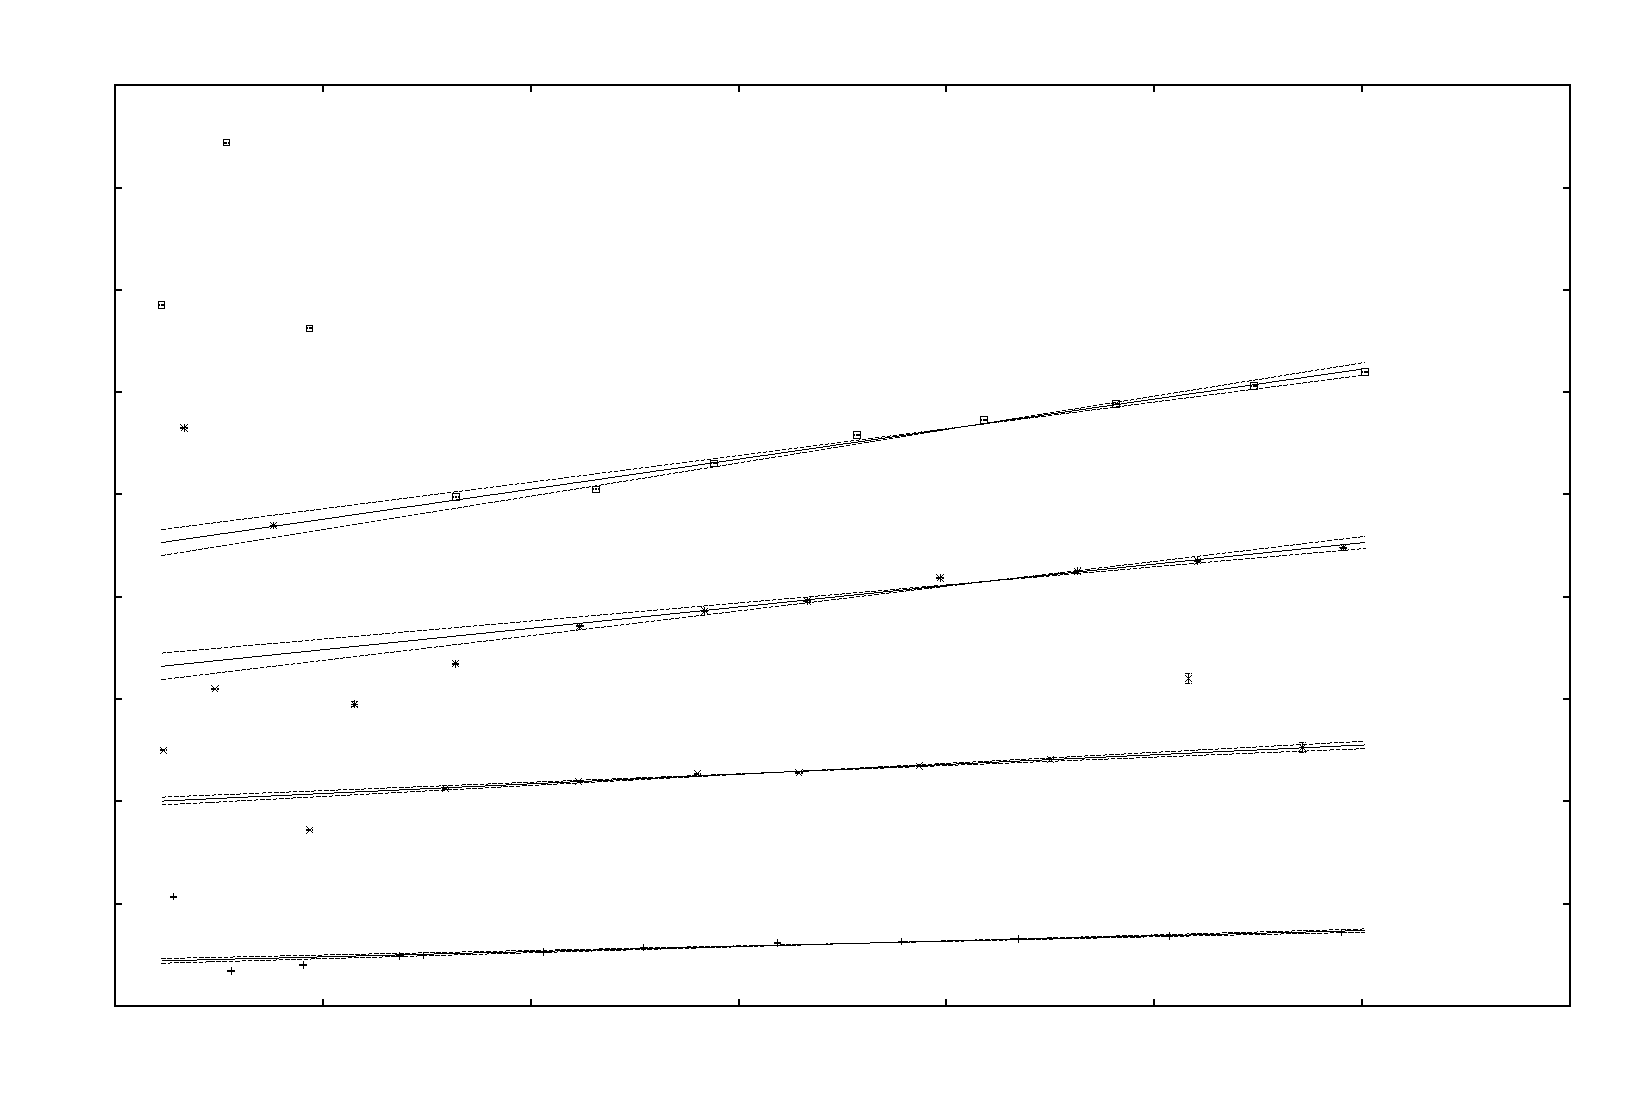
\includegraphics{plot-X}}%
    \gplfronttext
  \end{picture}%
\endgroup
